\section{Projektorganisation}
Die nachfolgenden Abschnitte beschreiben den organisatorischen Ablauf innerhalb der Projektgruppe. Dazu geh\"ort die Aufteilung in Gruppen, sowie die zeitliche Planung und Rollenverteilung. Des weiteren werden hier das Vorgehen f\"ur das gesamte Projekt und die verwendeten Werkzeuge beschrieben.

\subsection{Organisation der Teilgruppen (Materialfluss, Fahrzeuge, Simulation)}
Die Projektgruppe ist in die drei Teilgruppen unterteilt,  da das Gesamtprojekt in eindeutig abgrenzbare Aufgabenfelder gegliedert ist und so Kompetenzen und Verantwortlichkeiten klar definiert werden können. 

\begin{itemize}
\item \textbf{Materialfluss} \\
Die Teilgruppe Materialfluss befasst sich mit Programmierung der Sensorik und Aktorik für die Rampen, sowie dem Aufbau eines Sensornetzwerkes zur Kommunikation zwischen den verschiedenen Akteuren der Simulation. 

\item \textbf{Fahrzeuge} \\
Die Teilgruppe Fahrzeuge befasst sich mit allen Aspekten, die für das Funktionieren der Fahrzeuge verantwortlich sind. Dazu zählen unter anderem die Navigation, Odometrie und Lokalisierung. Auch ist die Einrichtung der Versorgungsinfrastruktur für die Fahrzeuge in Form von Ladestationen f\"allt in den Aufgabenbereich der Fahrzeuggruppe. Zusammen entwickeln die Teilgruppen Fahrzeuge und Materialfluss das physische System, so dass Kommunikation und Abstimmung zwischen diesen beiden Gruppen besonders wichtig sind. 

\item \textbf{Simualtion} \\
Die Teilgruppe Simulation entwickelt die Software mit der eine virtuelle Simulation erstellt wird. Diese Software beinhaltet einen hybriden Modus, in dem das physische System auf die Software abgebildet wird und beide Teilsysteme ein Gesamtsystem bilden. Für die Entwicklung des Hybridmodus muss ein funktionierendes physisches System vorliegen.
\end{itemize}

\subsection{Rollenverteilung}

Um organisatorische Aspekte innerhalb des Projektes besser umsetzen zu k\"onnen, wurden unterschiedliche Rollen definiert, die jeweils einen Bereich des Projektes abdecken sollen. Dazu geh\"oren folgende Aufgaben:

\begin{itemize}
\item\textbf{Administrator}

Der Administrator ist f\"ur die Einrichtung und Betreuung der Server und Tools zust\"andig, dazu z\"ahlt auch die Einrichtung der Webseite.

\item \textbf{Aussendarstellung}

Um das Projekt vern\"unftig zu Repr\"asentieren, verwalten die zust\"andigen der Aussendarstellung den Inhalt der Webseite. Ausserdem sind sie f\"ur die externen Kontakte und Events / Pr\"asentationen verantwortlich.

\item \textbf{Dokumentenbeauftragte}

Damit am Ende ein einheitliches Format f\"ur den Endbericht gilt, organisieren, sammeln und verwalten die Beauftragten jegliche Quellen und Berichte ( dazu z\"ahlt auch das Repository ). Des weiteren sind sie Ansprechpartner bei fragen zur Literatur.

\item \textbf{Gruppenleiter}

Da das Projekt aus drei Teilgruppen besteht, besitzt jede Gruppe einen eigenen Gruppenleiter, der die Prozesse innerhalb der Gruppe lenkt und gemeinsam mit den anderen Gruppenleitern das gesamte Projekt koordiniert.

\item \textbf{Qualit\"atsmanagement}

Damit der Projektplan eingehalten wird, ist es Aufgabe des Qualit\"atsmanagements, dass die Prozesse ( Scrums ) eingehalten und korrekt ausgef\"urt werden. Zus\"atzlich sind sie f\"ur die System und Integrationstests verantwortlich.

\item \textbf{Werkzeugbeauftragte}

Die Werkzeugbeauftragen verwalten die ben\"otigten Ger\"ate und Schl\"ussel f\"ur die gesamte Projektgruppe. Weiterhin regeln sie, mit R\"ucksprache mit den Betreuern, den Einkauf der Hardware und Software.

\end{itemize}


\subsection{Vorgehensmodell}
Für die Durchführung der Projektgruppe muss ein Vorgehensmodell, sowohl für die Gesamt- als auch für die Teilgruppen, festgelegt werden. Durch ein Vorgehensmodell wird die Arbeit im Team strukturiert und es wird festgelegt, wie bestimmte Aufgaben, wie z.B. Abgleich mit Kunden und Anwendern, umgesetzt werden sollen. Sowohl für die Teilgruppen als auch für die Gesamtgruppe wurde ein Scrummodell als Vorgehensmodell gewählt ( siehe Abbildung 9).

	\begin{figure}[h!]
		\centering
			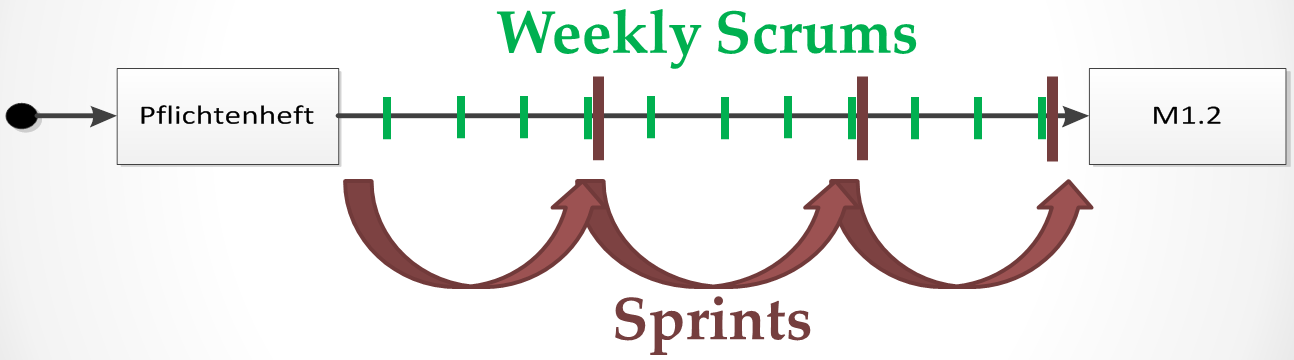
\includegraphics[width=0.9\textwidth]{Projektorganisation_Scrum.png}
			\caption{Scrumplanung f\"ur einen Meilenstein}
			\label{Projektorganisation Scrum}
	\end{figure}	

Da es für ein sehr komplexes Projekt, wie das vorliegende, schwierig ist nur von einer groben Vision, sowie von User Stories auszugehen, wurden zun\"achst auf Basis des vorliegenden Lastenhefts in jeder Teilgruppe Pflichtenhefte erstellt. Anschließend wurden die dazugeh\"origen User Stories definiert, die die Anforderungen aus dem Pflichtenheft ber\"ucksichtigen und aus Anwendersicht darstellen. Die Sprints in den Teilgruppen sind mit einem Monat bemessen und werden zur Durchf\"uhrung der User Stories genutzt. Die Rolle des Product Owners wird von den beiden Betreuern eingenommen, die sowohl für die Teil- als auch für die Gesamtgruppen zur Verfügung stehen, um die entwickelten Funktionalit\"aten abzugleichen.
Die Durchf\"uhrung von Daily Scrums ist zeitlich nicht m\"oglich, da es sich um eine studentische Projektgruppe handelt, deren Stundenplan keine t\"aglichen Treffen erm\"oglicht. Deshalb wurde das Scrum Vorgehensmodell dahingehend angepasst, dass die Daily Scrums in Weekly Scrums abgewandelt wurden. Die Weekly Scrums finden sowohl in den Teilgruppen als auch in der Gesamtgruppe statt. In den Weekly Scrums der Gesamtgruppe wird zun\"achst von jeder Person berichtet, welche Aufgaben in der vorherigen Woche erledigt wurden, damit entstandene Probleme und Hindernisse direkt in der Gruppe besprochen und eventuell beseitigt werden k\"onnen. Die Ergebnisse aus den Teilgruppen werden ebenfalls vorgestellt und mit den Product Ownern abgeglichen.
Das Scrum Vorgehensmodell wird mit  Prototyping kombiniert ( siehe Abbildung 10 ).

Durch das Prototyping sollen zu bestimmten Meilensteinen die kombinierten Ergebnisse aus den Teilgruppen vorgestellt werden, um den Stand des Gesamtsystems begutachten zu k\"onnen. Betrachtet man das gesamte Projekt, so besteht es aus 2 Prototyping Phasen. Diese trennen sich im zweiten Meilenstein. Bis zu diesem Zeitpunkt wird mit horizontalen Prototyping die Basis des Projektes geschaffen. Das bedeutet, dass alle Grundfunktionalit\"aten implementiert und umgesetzt werden. Danach folgt das vertikale Prototyping in dem die Funktionalit\"aten um weitere Aspekte und Feinheiten er\"anzt werden. Innerhalb dieser beiden Phasen kommt es immer wieder zu Aufgabenbereichen, die jede Teilgruppe f\"ur sich umsetzt. Ebenfalls sind Phasen vorhanden, in denen die Ergebnisse der einzelnen Gruppen zusammengef\"uhrt werden m\"ussen, wodurch das Zusammenspiel zwischen dem Materialfluss und der Volksbots, sowie die Darstellung in der Simulation, entsteht.

	\begin{figure}[h!]
		\centering
			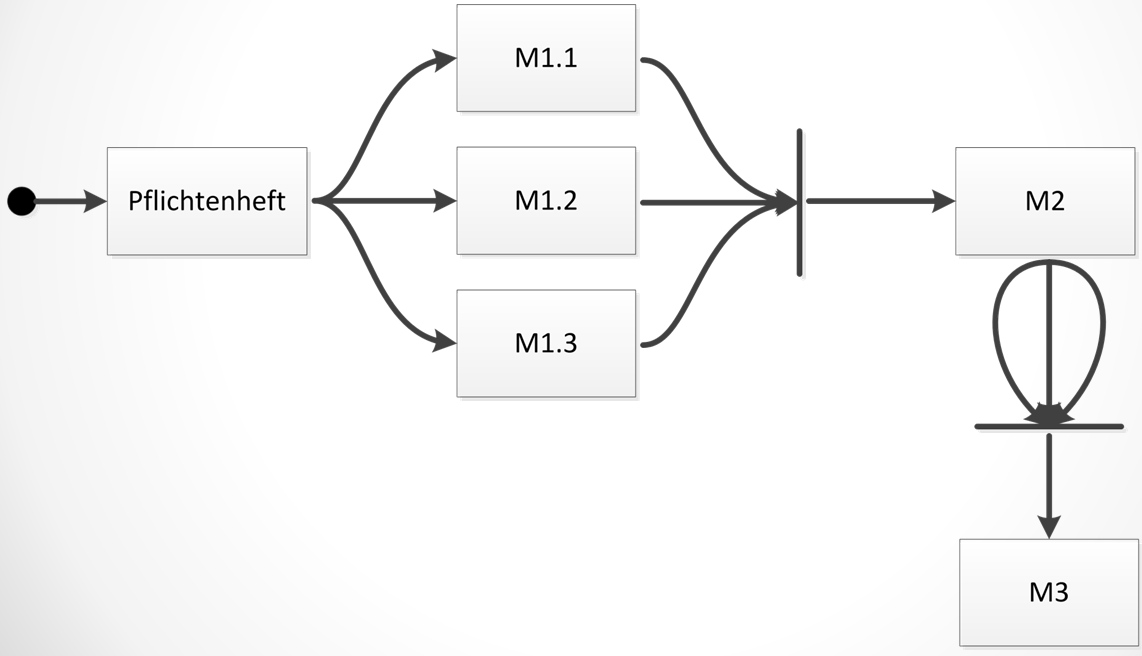
\includegraphics[width=0.9\textwidth]{Vorgehensmodell_Prototyping.png}
			\caption{Modell für die Darstellung der einzelnen Projektphasen}
			\label{Vorgehensmodell_Prototyping}
	\end{figure}	
